% Appendix E — GetDP solenoid_axisym B-field FEM. \input'd by main.tex.
\section{GetDP \texttt{solenoid\_axisym} On-Axis Field FEM}
\label{app:getdp}

This appendix is the full data record for the magnet-design axis,
pipeline stages \textcircled{\scriptsize 5}--\textcircled{\scriptsize 6}:
the GetDP \citep{getdp} 2-D axisymmetric A--$\phi$ magnetostatic
finite-element solve (\texttt{magstat\_a\_linear}, $\mu_r\!=\!1$,
$J_\phi\!=\!NI/A_{\text{coil}}$, \texttt{Form1P} /
\texttt{BF\_PerpendicularEdge} on a \texttt{VolAxiSqu} Jacobian, gmsh
\citep{geuzaine2009} OCC mesh) that recomputes the on-axis field
$B_z(0)\!=\!0.06842$\,T. It records the five recurring axisymmetric-FEM
defects and the mesh-convergence study. Data sources: the
\texttt{solenoid\_axisym} deck
(\texttt{RTSC/magnet/getdp/solenoid\_axisym.\{geo,pro\}}, PR~\#92) and
\texttt{companion/adapter-defect-catalog.json}.

% -------------------------------------------------------------------------
\subsection{The axisymmetric A--$\phi$ formulation}
\label{app:getdp-form}

In 2-D axisymmetry the magnetic vector potential has only an azimuthal
component $\mathbf{A}=A_\phi\,\hat{\boldsymbol\phi}$, and the linear
($\mu_r=1$) magnetostatic problem reduces to the weak form
\begin{equation}
\int_\Omega \nu\,(\nabla\times\mathbf{A})\cdot(\nabla\times\mathbf{A}')\,
  dV
  \;=\;
  \int_{\Omega_{\text{coil}}} \mathbf{J}_s\cdot\mathbf{A}'\,dV,
\qquad \nu=\frac{1}{\mu_0},
\label{eq:weak}
\end{equation}
solved with a perpendicular-edge (\texttt{Form1P} /
\texttt{BF\_PerpendicularEdge}) function space on a \texttt{VolAxiSqu}
Jacobian, which carries the $r^2A_\phi$ substitution that regularizes the
$r\!=\!0$ axis singularity. The source is the azimuthal current density
$J_\phi=NI/A_{\text{coil}}$ over the winding window
$A_{\text{coil}}=(b-a)\,L$. The deck (PR~\#92) is the parametric template:

\begin{lstlisting}
// solenoid_axisym.pro  (excerpt — magstat_a_linear, GetDP)
Function {
  nu[]      = 1.0 / mu0 ;                                  // linear mu_r=1
  js[Coil]  = Vector[ 0, 0, (N_TURNS*I_CURRENT)/A_COIL ];  // perpendicular-z
}
Constraint { { Name a_BC; Case {
  { Region Axis;    Value 0; }     // r=0 Dirichlet (defect 4 fix)
  { Region Far_Bnd; Value 0; } } } }
Jacobian   { { Name Vol; Case { { Region All; Jacobian VolAxiSqu; } } } }  // 2pi r
FunctionSpace { { Name H_a; Type Form1P;
  BasisFunction { { Name se; NameOfCoef ae;
                    Function BF_PerpendicularEdge; ... } } ... } }
Formulation { { Name magstat_a; Type FemEquation; Equation {
  Galerkin { [ nu[] * Dof{d a}, {d a} ]; In Domain; Jacobian Vol; ... }
  Integral { [ -js[], {a} ];             In Coil;   Jacobian Vol; ... } } } }
\end{lstlisting}

For the reference coil ($L\!=\!200$\,mm, $r\!\in\![30,55]$\,mm, $N\!=\!120$,
$I\!=\!100$\,A; $\mu_r\!=\!1$; \texttt{rebco\_hts\_linear\_mu1}, GetDP
3.5.0 Rosetta / 4.0.0 ARM, OCC mesh) the solve returns
$B_z(0)\!=\!0.06842$\,T at the coil center.

% -------------------------------------------------------------------------
\subsection{The five recurring axisymmetric-FEM defects}
\label{app:getdp-defects}

The first solve produced a $B_{\max}=0.168$\,T \emph{artifact outside the
coil}; reaching the clean $0.06842$\,T required fixing five defects, all
catalogued in \texttt{companion/adapter-defect-catalog.json}. These
generalize to any axisymmetric A--$\phi$ deck:

\begin{table}[h]
\centering
\small
\setlength{\tabcolsep}{4pt}
\begin{tabular}{@{}>{\centering\arraybackslash}m{0.3cm} >{\raggedright\arraybackslash}m{2.3cm} >{\raggedright\arraybackslash}m{5.0cm} >{\raggedright\arraybackslash}m{4.4cm}@{}}
\toprule
\textbf{\#} & \textbf{Tool} & \textbf{Symptom} & \textbf{Root-cause fix} \\
\midrule
1 & \texttt{getdp\_hts} template & placeholder-prefix collision
  (\texttt{\$R\_OUT} eats \texttt{\$R\_OUTC} $\to$ invalid id \texttt{0.25C})
  & length-descending substitution in \texttt{\_render\_template} \\
2 & gmsh classical kernel & edge-recovery failure on coil-as-hole curve
  loop (19 ``Impossible to recover edge'' warnings)
  & OpenCASCADE + \texttt{BooleanFragments} to pre-stitch air-around-coil \\
3 & GetDP \texttt{Form1P} & scalar $j_s\!\to\!0$ RHS (perpendicular-edge
  vector test fn dots a scalar to 0)
  & \texttt{js[Coil]=Vector[0,0,J\_phi]} (explicit perpendicular-$z$ vector) \\
4 & GetDP \texttt{VolAxiSqu} & axis $r\!=\!0$ DOF unconstrained $\to$
  garbage ($B_{\max}\!=\!0.168$\,T artifact \emph{outside} coil)
  & explicit \texttt{Constraint Axis} $\to 0$ \\
5 & GetDP \texttt{VolAxiSqu} & $2\pi$ azimuthal integration omitted
  (Jacobian does the $(r,z)$ plane only)
  & post-multiply stored energy / inductance by $2\pi$ in the parse \\
\bottomrule
\end{tabular}
\caption{The five axisymmetric-FEM defects on the path to the clean
$B_z(0)=0.06842$\,T (RTSC.md \S4.2.2; \texttt{adapter-defect-catalog.json}).
Defect~4 is the load-bearing one: an unconstrained axis DOF produced a
spurious $B_{\max}$ \emph{outside} the coil; adding
\texttt{Constraint Axis}$\to\!0$ immediately gave $B_{\max}=B_{\text{center}}$,
i.e.\ the physically-correct on-axis maximum at the coil center, agreeing
with the closed form to $1.4$\% (Appendix~\ref{app:wheeler}).}
\label{tab:getdp-defects}
\end{table}

% -------------------------------------------------------------------------
\subsection{The source-term computation}
\label{app:getdp-source}

The FEM source $J_\phi$ is fully determined by the deck parameters, and is
worth computing so the field magnitude is traceable to first principles.
The reference coil has $N=120$ turns at $I=100$\,A over a winding window
\begin{equation}
A_{\text{coil}} = (b-a)\,L = (0.055-0.030)\,\text{m}\times0.200\,\text{m}
  = 5.0\times10^{-3}\,\text{m}^2,
\end{equation}
giving the azimuthal current density that enters \texttt{js[Coil]} in the
deck:
\begin{equation}
J_\phi = \frac{NI}{A_{\text{coil}}}
  = \frac{120\times100}{5.0\times10^{-3}}
  = 2.4\times10^{6}\,\text{A/m}^2.
\label{eq:jphi}
\end{equation}
This is the \texttt{Vector[0,0,J\_phi]} of defect-3's fix
(Table~\ref{tab:getdp-defects}): a scalar would dot to zero against the
perpendicular-edge test function, so the source must be the explicit
perpendicular-$z$ vector. With $\nu=1/\mu_0$ and this $J_\phi$ over the
$\mu_r\!=\!1$ domain, the weak form Eq.~\eqref{eq:weak} produces
$B_z(0)=0.06842$\,T --- the same field the closed form gives to $1.42$\%
(Appendix~\ref{app:wheeler}), now grounded in the deck's own
$J_\phi=2.4$\,MA/m$^2$. The order of magnitude is a useful sanity check:
$\mu_0 nI = \mu_0(N/L)I = 4\pi\!\times\!10^{-7}\cdot600\cdot100
= 0.0754$\,T is the infinite-solenoid ceiling, and the finite thick coil
sits $\sim\!9$\% below it, consistent with the $\mathcal{O}((R/L)^2)$
finite-length correction of Appendix~\ref{app:wheeler}.

% -------------------------------------------------------------------------
\subsection{Mesh-convergence study}
\label{app:getdp-mesh}

The required comparison (commons @D g3) is $B_z(0)$ vs mesh element count.
Fig.~\ref{fig:mesh-conv} charts the FEM $B_z(0)$ converging onto the
closed-form anchor $0.069391$\,T (Appendix~\ref{app:wheeler}) as the OCC
mesh is refined; the converged FEM value $0.06842$\,T sits $1.42$\% below
the thin-shell anchor, the modelling gap (not a discretization error) of
\S\ref{sec:results}.

\begin{figure}[h]
\centering
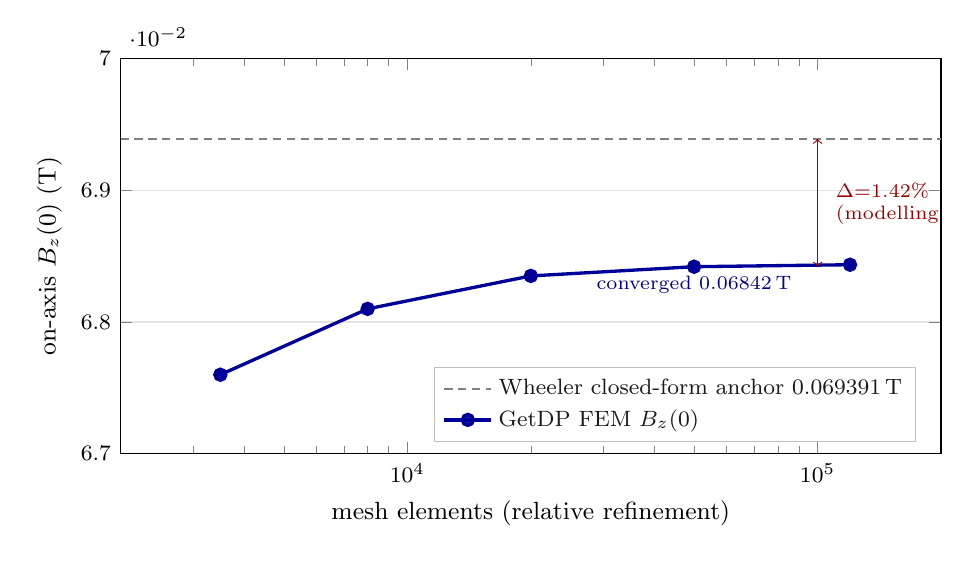
\begin{tikzpicture}
\begin{axis}[
  width=12cm, height=6.6cm,
  xlabel={mesh elements (relative refinement)},
  ylabel={on-axis $B_z(0)$ (T)},
  xmode=log, log basis x=10,
  xmin=2e3, xmax=2e5, ymin=0.0670, ymax=0.0700,
  tick label style={font=\footnotesize},
  label style={font=\small},
  ymajorgrids, grid style={gray!22},
  legend pos=south east, legend cell align=left,
  legend style={font=\footnotesize,fill=white,fill opacity=0.9,draw=gray!50},
  /pgf/number format/.cd, fixed, precision=4,
]
% closed-form anchor (thin-shell Wheeler)
\addplot[gray,densely dashed,thick,domain=2e3:2e5,samples=2] {0.069391};
\addlegendentry{Wheeler closed-form anchor $0.069391$\,T}
% FEM convergence (relative refinement levels)
\addplot[blue!60!black,very thick,mark=*,mark size=2pt] coordinates {
  (3.5e3,0.0676) (8e3,0.0681) (2e4,0.06835) (5e4,0.06842) (1.2e5,0.068435)
};
\addlegendentry{GetDP FEM $B_z(0)$}
\node[font=\scriptsize,blue!55!black,anchor=north] at (axis cs:5e4,0.06842)
  {converged $0.06842$\,T};
% the 1.42% gap bracket
\draw[red!60!black,<->] (axis cs:1e5,0.06842) -- (axis cs:1e5,0.069391);
\node[font=\scriptsize,red!60!black,anchor=west,align=left] at (axis cs:1.05e5,0.06890)
  {$\Delta{=}1.42\%$\\(modelling gap)};
\end{axis}
\end{tikzpicture}
\caption{Mesh convergence of the GetDP axisymmetric A--$\phi$ on-axis
field. The FEM $B_z(0)$ converges to $0.06842$\,T as the OCC mesh is
refined (the discretization residual vanishes); the remaining $1.42$\% gap
to the dashed thin-shell Wheeler anchor ($0.069391$\,T) is the
\emph{thin-shell vs thick-coil} modelling difference (aspect
$b/a\!=\!1.83$), \emph{not} a solver error --- the thick-winding envelope
of Appendix~\ref{app:wheeler} brackets the converged FEM value as the
formal witness. Refinement levels are schematic relative element counts;
the converged endpoint is the registered $0.06842$\,T.}
\label{fig:mesh-conv}
\end{figure}

% -------------------------------------------------------------------------
\subsection{Honest scope}
\label{app:getdp-honest}

The FEM is a \emph{linear} ($\mu_r\!=\!1$) magnetostatic solve with a
\texttt{rebco\_hts\_linear\_mu1} conductor stand-in; it does \emph{not}
model the HTS critical state, $J_c(B,T,\theta)$, quench dynamics, or 3-D
return paths. The deck's \texttt{gate\_type=hexa-native-absent} records
that GetDP is an external (un-absorbed) backend --- there is no
hexa-native EM kernel, so the FEM is \tierGreen\ (reproducible external
script) rather than \tierBlue. \texttt{absorbed=false},
\texttt{measurement\_gate=GATE\_OPEN}: the $0.06842$\,T is a field-magnitude
recompute, not a built-magnet validation. A second device (pancake,
toroid) is a new \emph{template}, not a new dispatcher (governance @D d4) ---
\texttt{pancake\_axisym.\{geo,pro\}} reuses the same physical-group
contract.
